\documentclass[a4paper,11pt]{article}
\usepackage{amsmath,amsthm,amsfonts,amssymb,amscd,amstext,vmargin,graphics,graphicx,tabularx,multicol} 
\usepackage[francais]{babel}
\usepackage[utf8]{inputenc}  
\usepackage[T1]{fontenc} 
\usepackage{pstricks-add,tikz,tkz-tab,variations}
\usepackage[autolanguage,np]{numprint} 

\setmarginsrb{1.5cm}{0.5cm}{1cm}{0.5cm}{0cm}{0cm}{0cm}{0cm} %Gauche, haut, droite, haut
\newcounter{numexo}
\newcommand{\exo}[1]{\stepcounter{numexo}\noindent{\bf Exercice~\thenumexo} : \marginpar{\hfill /#1}}
\reversemarginpar


\newcounter{enumtabi}
\newcounter{enumtaba}
\newcommand{\q}{\stepcounter{enumtabi} \theenumtabi.  }
\newcommand{\qa}{\stepcounter{enumtaba} (\alph{enumtaba}) }
\newcommand{\initq}{\setcounter{enumtabi}{0}}
\newcommand{\initqa}{\setcounter{enumtaba}{0}}

\newcommand{\be}{\begin{enumerate}}
\newcommand{\ee}{\end{enumerate}}
\newcommand{\bi}{\begin{itemize}}
\newcommand{\ei}{\end{itemize}}
\newcommand{\bp}{\begin{pspicture*}}
\newcommand{\ep}{\end{pspicture*}}
\newcommand{\bt}{\begin{tabular}}
\newcommand{\et}{\end{tabular}}
\renewcommand{\tabularxcolumn}[1]{>{\centering}m{#1}} %(colonne m{} centrée, au lieu de p par défault) 
\newcommand{\tnl}{\tabularnewline}

\newcommand{\trait}{\noindent \rule{\linewidth}{0.2mm}}
\newcommand{\hs}[1]{\hspace{#1}}
\newcommand{\vs}[1]{\vspace{#1}}

\newcommand{\N}{\mathbb{N}}
\newcommand{\Z}{\mathbb{Z}}
\newcommand{\R}{\mathbb{R}}
\newcommand{\C}{\mathbb{C}}
\newcommand{\Dcal}{\mathcal{D}}
\newcommand{\Ccal}{\mathcal{C}}
\newcommand{\mc}{\mathcal}

\newcommand{\vect}[1]{\overrightarrow{#1}}
\newcommand{\ds}{\displaystyle}
\newcommand{\eq}{\quad \Leftrightarrow \quad}
\newcommand{\vecti}{\vec{\imath}}
\newcommand{\vectj}{\vec{\jmath}}
\newcommand{\Oij}{(O;\vec{\imath}, \vec{\jmath})}
\newcommand{\OIJ}{(O;I,J)}


\newcommand{\bmul}[1]{\begin{multicols}{#1}}
\newcommand{\emul}{\end{multicols}}

\newcommand{\reponse}[1][1]{%
\multido{}{#1}{\makebox[\linewidth]{\rule[0pt]{0pt}{20pt}\dotfill}
}}

\newcommand{\titre}[5] 
% #1: titre #2: haut gauche #3: bas gauche #4: haut droite #5: bas droite
{
\noindent #2 \hfill #4 \\
#3 \hfill #5

\vspace{-1.6cm}

\begin{center}\rule{6cm}{0.5mm}\end{center}
\vspace{0.2cm}
\begin{center}{\large{\textbf{#1}}}\end{center}
\begin{center}\rule{6cm}{0.5mm}\end{center}
}



\begin{document}
\pagestyle{empty}
\titre{Interrogation : Proportionnalité, pourcentages et échelles}{Nom :}{Prénom :}{Classe}{Date}

\exo{2}\\

\bmul{2}
\qa Un grand magasin vend des agendas tous au même prix. A l'aide du produit en croix, trouver le prix $x$ manquant dans le tableau suivant :\\

\columnbreak

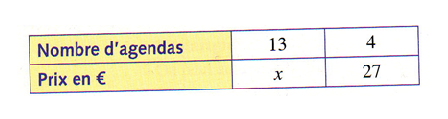
\includegraphics[scale=1]{tab1.eps} 

\emul

\noindent \reponse[3]\\

\qa Avec 250 g de café, on peut préparer 30 expresso. \\
Quelle masse de café faut-il pour préparer 22 expresso ?\\
\reponse[4]\\



\exo{2}\\
\initq 
\q \textit{"Dans les années 2 000, plus\textbf{ des trois quart} des véhicules neufs immatriculés en France était des diesel. Cependant, depuis deux ans les choses bougent à la baisse. Seulement \textbf{5 français sur 10} achèteraient du diesel."}\\

 \textbf{Compléter le texte avec des pourcentages :} \\
 
"Dans les années 2 000, plus ........................................... des véhicules neufs immatriculés en France était des diesel. Cependant, depuis deux ans les choses bougent à la baisse. Seulement .......................................... des français achèteraient du diesel."\\

\q Calculer des pourcentages :\\

\bmul{2}

\initqa \qa 45 $\%$ de 114 euros\\
\reponse[2]

\columnbreak

\qa 121 $\%$ de 205 L\\
\reponse[2]\\

\emul

\exo{1,5}

Le volume d'eau sur Terre est d'environ 1 830 millions de $km^{3}$. \\
97,1 $\%$ de ce volume est composé d'eau salée.\\

Calculer le volume d'eau douce sur terre.\\
\reponse[4]\\

\newpage


\exo{2,5}
\begin{center}
\includegraphics[scale=0.65]{carteechelle.eps} 
\end{center}
\begin{flushright}
L'échelle : $\dfrac{1}{\text{20 000 000}}$.
\end{flushright}


\initq \q Quelle est la distance réelle, en km,entre Lille et Strasbourg? (Justifier votre réponse par un calcul)\\
\reponse[3]\\

\q Placer sur cette carte, la ville de Paris, située à 490 km de Strasbourg et à 750 km de Montpellier.(Justifier votre réponse par des calculs)\\
\reponse[4]\\

\exo{2}
Voici une photo à l'échelle $\dfrac{1}{145}$ du tableau \textit{Guernica} peint en 1937 par Pablo Picasso et représentant une scène de massacre dans la ville de Guernica pendant la guerre civile espagnole.

\begin{center}
\includegraphics[scale=1]{proportionnalite3.eps} 

\end{center}

$\rightarrow$ Quelles sont les dimensions réelles de ce tableau ?\\
\noindent \reponse[4]

\end{document}
